
\section{Results}
\subsection{Six DOF Stewart Platform}
As earlier mentioned, the Stewart platform has already been designed and fabricated and our part in this work was to do an evaluation of the same to verify its mechanical feasibility. As such, the various parts of the platform were obtained and assembled. For further analysis, a 3D model of the same platform was done using Autodesk Inventor.

The assembled Stewart platform is as shown in figure \ref{fig}. Figure \ref{fig1} shows the Stewart platform configuration setup with the Wind tunnel's test section.
\begin{center}
	\begin{figure}[H]
		\centering
		\includegraphics[width=0.6\linewidth]{Figures/stew_asm.jpg}
		\caption[Assembled Platform]{Assembly of Stewart Platform}
		\label{fig}
	\end{figure}
\end{center}
\begin{center}
	\begin{figure}[H]
		\centering
		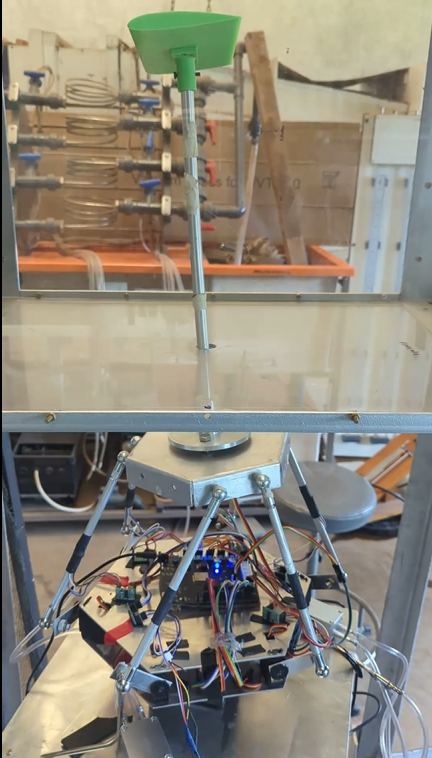
\includegraphics[width=0.7\linewidth]{Figures/stew_wind1.png}
		\caption[Model placement in Test Section]{Stewart platform and Test section configuration}
		\label{fig1}
	\end{figure}
\end{center}

\subsection{Force Measurement by the Stewart Platform}
Finite Element Analysis done on FEA environment in Autodesk inventor showed expected strain values on each
Stewart platform leg as shown in figure \ref{strain}.

\begin{center}
	\begin{figure}[H]
		\centering
		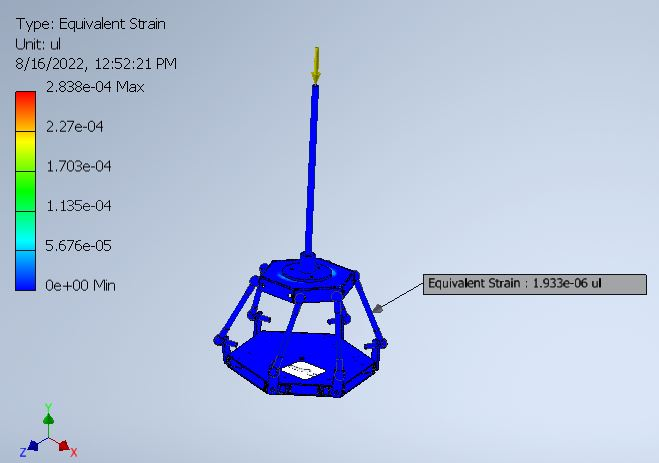
\includegraphics[width=0.6\linewidth]{Figures/Equivalent}
		\caption[Equivalent strain]{Strain induced on each of the legs}
		\label{strain}
	\end{figure}
\end{center}
These strains are small thus they need amplification in order provide
 substantial input to be used for force measurements. Strain values detected on the legs and amplified by the
 HX711s were obtained and displayed on the HMI as force measurements when load is applied on the platform.
\subsection{Human Machine Interface}
The user interface of the platform was programmed using golang and this resulted in the view below with the use of sliders for platform positioning and buttons to set model orientations and start data collection.
\begin{center}
	\begin{figure}[H]
		\centering
		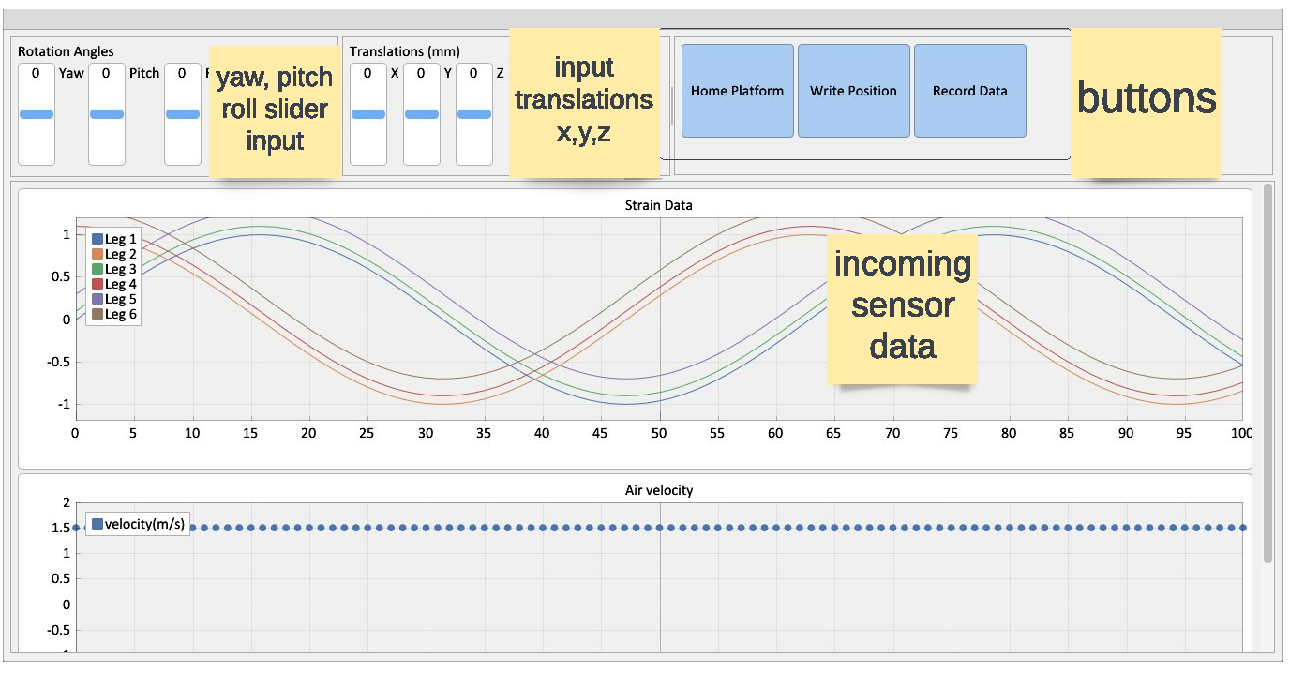
\includegraphics[width=1\linewidth]{Figures/hmi}
		\caption[HMI Dashboard]{HMI Dashboard}
	\end{figure}
\end{center}

This includes slider buttons to control platform position and orientation. It also includes buttons to allow for data capture  and platform control. The dashboard also has a live plot of incoming data to provide immediate user feedback.

The transport via TCP to the microcontroller was also tested, it showed bidirectional streaming of data to and from the microcontroller making it suitable for communication.

\subsection{PCB}
The schematics from the electrical designs as seen in the appendix were routed to generate a PCB ready for manufacture. This is shown in the 3D render below:
\begin{center}
	\begin{figure}[H]
		\centering
		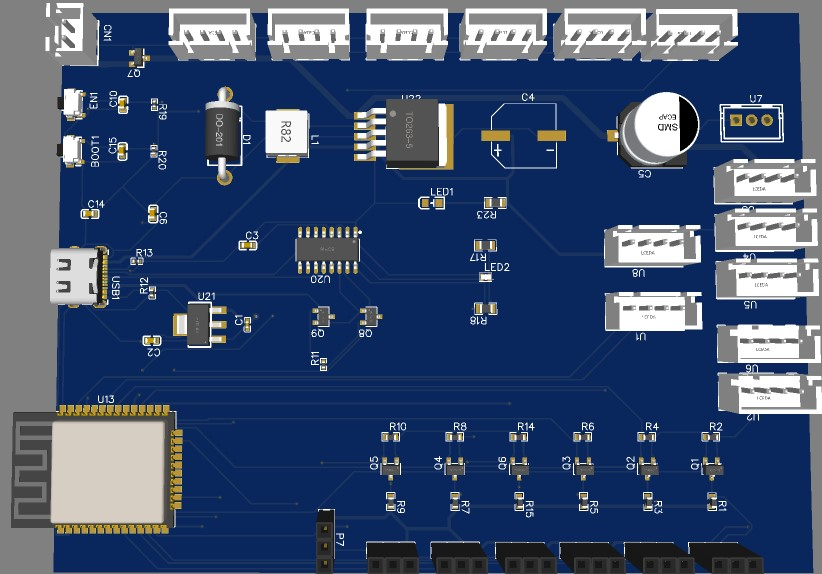
\includegraphics[width=0.7\linewidth]{Figures/pcb}
		\caption[Printed Circuit Board view]{Printed Circuit Board view}
		\label{fig:pcb3d}
	\end{figure}
\end{center}
The PCB is meant to be compact as shown in the figure \ref{fig:pcb3d}. It is also integrates most of the components to minimize use of wires to make connections.

\subsection{Smoke Visualization}
The smoke emitting device was 3D printed and assembled into the wind tunnel as shown in \ref{fig:smoke_res}.
The device was able to create streamlines of smoke to improve visibility in the wind tunnel.
\begin{center}
	\begin{figure}
		\centering
		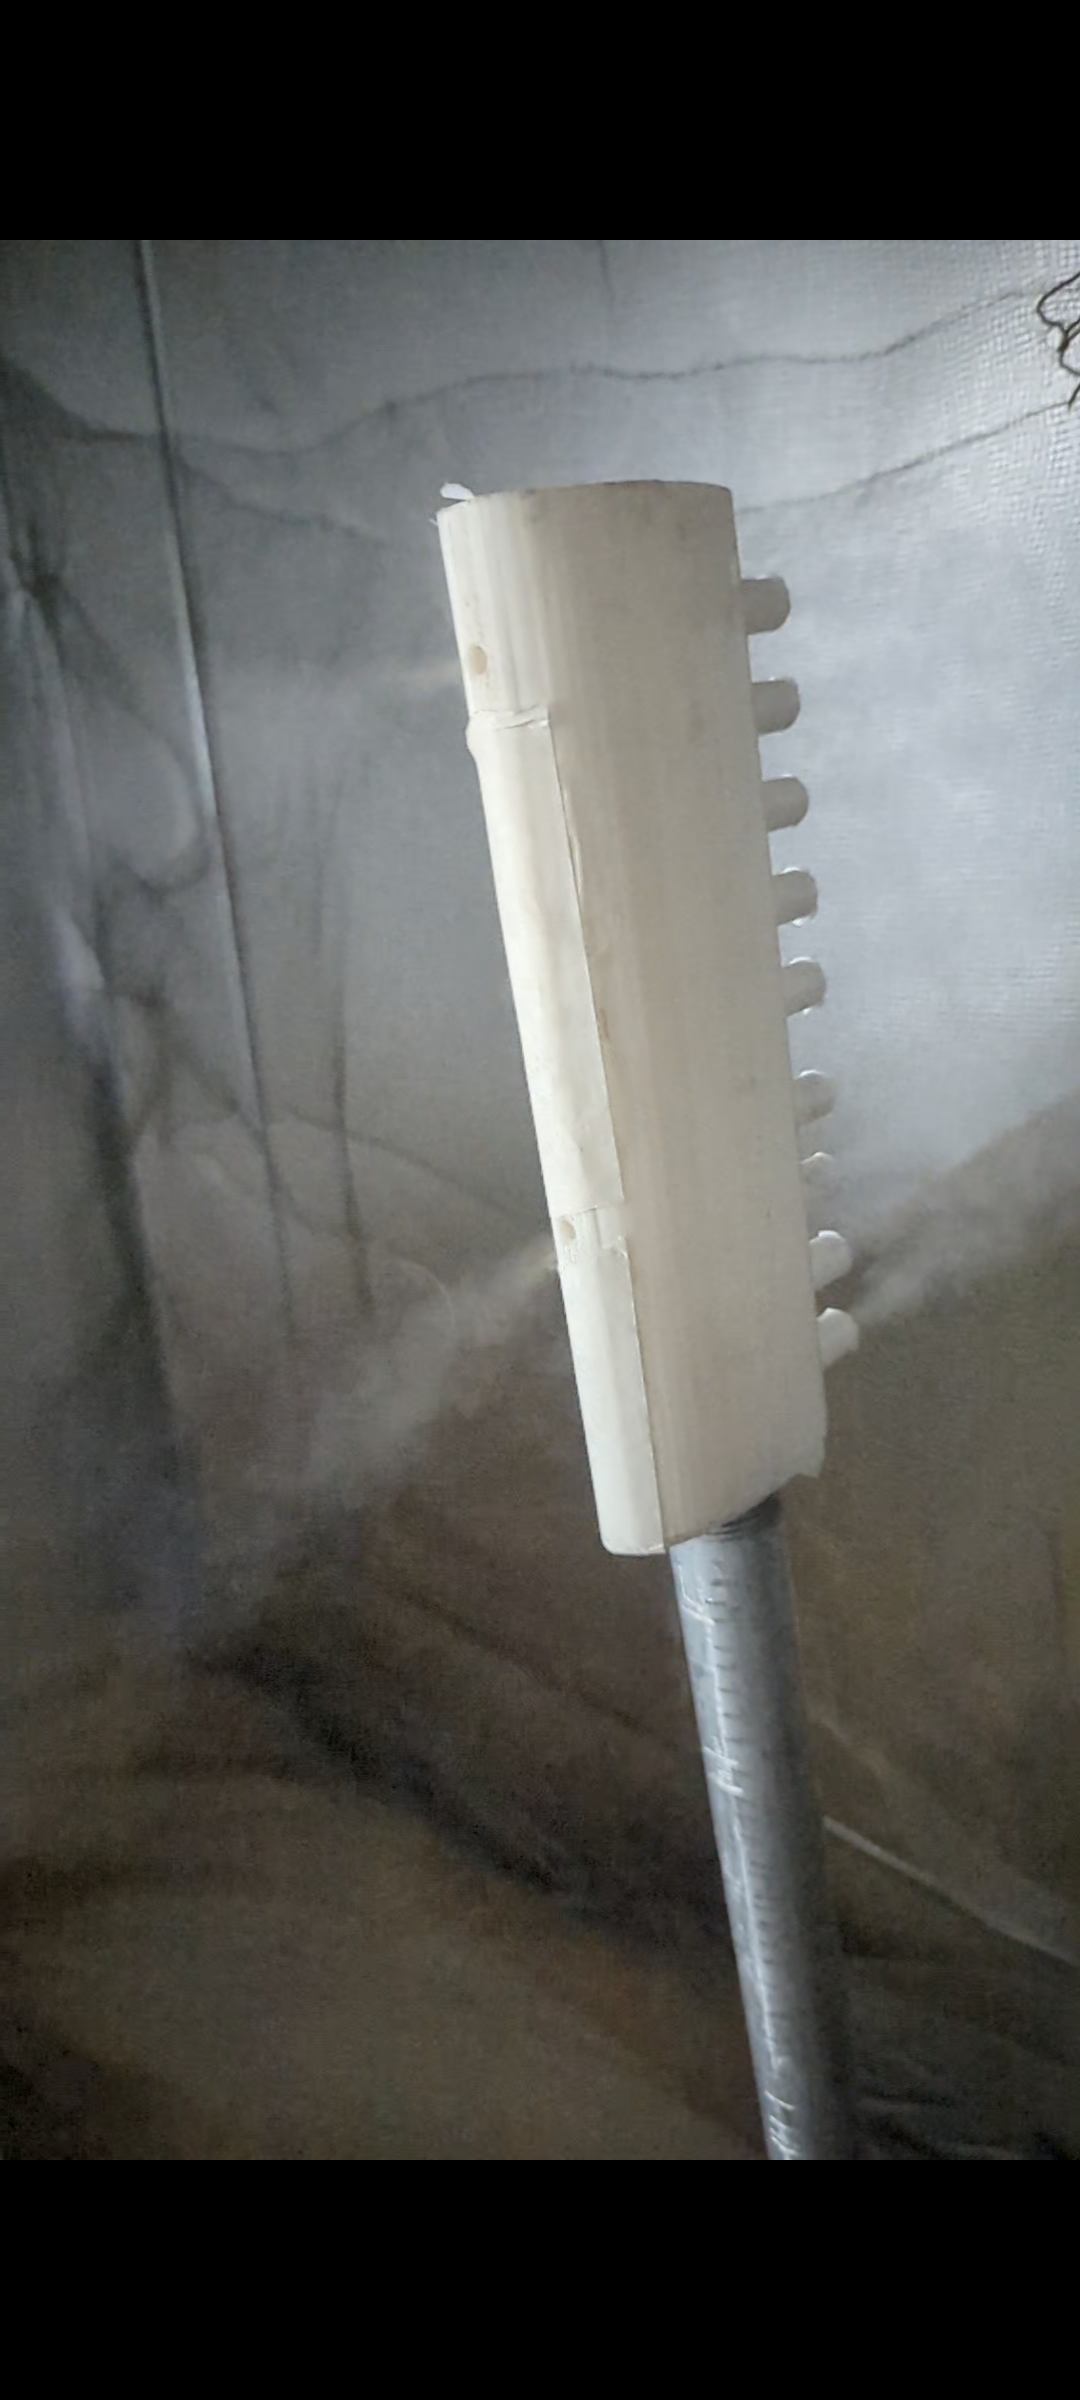
\includegraphics[width=0.5\linewidth]{Figures/Screenshot_20221211-185935.png}
		\caption[Smoke Emitting Device]{Smoke Emitting Device}
		\label{fig:smoke_res}
	\end{figure}
\end{center}
